\documentclass[a4paper, 11pt, notitlepage, english]{article}

\usepackage{babel}
\usepackage[utf8]{inputenc}
\usepackage[T1]{fontenc, url}
\usepackage{textcomp}
\usepackage{amsmath, amssymb}
\usepackage{amsbsy, amsfonts}
\usepackage{graphicx, color}
\usepackage{parskip}
\usepackage{framed}
\usepackage{amsmath}
\usepackage{xcolor}
\usepackage{multicol}
\usepackage{url}
\usepackage{flafter}


\usepackage{geometry}
\geometry{headheight=0.01mm}
\geometry{top=24mm, bottom=30mm, left=39mm, right=39mm}

%
% Parametere for inkludering av kode fra fil
%
\usepackage{listings}
\lstset{language=python}
\lstset{basicstyle=\ttfamily\small}
\lstset{frame=single}
\lstset{keywordstyle=\color{red}\bfseries}
\lstset{commentstyle=\itshape\color{blue}}
\lstset{showspaces=false}
\lstset{showstringspaces=false}
\lstset{showtabs=false}
\lstset{breaklines}

%
% Definering av egne kommandoer og miljøer
%
\newcommand{\dd}[1]{\ \text{d}#1}
\newcommand{\f}[2]{\frac{#1}{#2}} 
\newcommand{\beq}{\begin{equation*}}
\newcommand{\eeq}{\end{equation*}}
\newcommand{\bra}[1]{\langle #1|}
\newcommand{\ket}[1]{|#1 \rangle}
\newcommand{\braket}[2]{\langle #1 | #2 \rangle}
\newcommand{\braup}[1]{\langle #1 \left|\uparrow\rangle\right.}
\newcommand{\bradown}[1]{\langle #1 \left|\downarrow\rangle\right.}
\newcommand{\av}[1]{\left| #1 \right|}
\newcommand{\op}[1]{\hat{#1}}
\newcommand{\braopket}[3]{\langle #1 | {#2} | #3 \rangle}
\newcommand{\ketbra}[2]{\ket{#1}\bra{#2}}
\newcommand{\pp}[1]{\frac{\partial}{\partial #1}}
\newcommand{\ppn}[1]{\frac{\partial^2}{\partial #1^2}}
\newcommand{\up}{\left|\uparrow\rangle\right.}
\newcommand{\upup}{\left|\uparrow\uparrow\rangle\right.}
\newcommand{\down}{\left|\downarrow\rangle\right.}
\newcommand{\downdown}{\left|\downarrow\downarrow\rangle\right.}
\newcommand{\updown}{\left|\uparrow\downarrow\rangle\right.}
\newcommand{\downup}{\left|\downarrow\uparrow\rangle\right.}
\newcommand{\bupup}{\left.\langle\uparrow\uparrow\right|}
\newcommand{\bdowndown}{\left.\langle\downarrow\downarrow\right|}
\newcommand{\bupdown}{\left.\langle\uparrow\downarrow\right|}
\newcommand{\bdownup}{\left.\langle\downarrow\uparrow\right|}
\renewcommand{\d}{{\rm d}}
\newcommand{\Res}[2]{{\rm Res}(#1;#2)}
\newcommand{\To}{\quad\Rightarrow\quad}
\newcommand{\eps}{\epsilon}
\makeatletter
\renewcommand*\env@matrix[1][*\c@MaxMatrixCols c]{%
  \hskip -\arraycolsep
  \let\@ifnextchar\new@ifnextchar
  \array{#1}}
\makeatother

\renewcommand{\arraystretch}{2}
\setlength{\tabcolsep}{12pt}
\makeatletter
\renewcommand*\env@matrix[1][*\c@MaxMatrixCols c]{%
  \hskip -\arraycolsep
  \let\@ifnextchar\new@ifnextchar
  \array{#1}}
\makeatother

\newcommand{\bt}[1]{\boldsymbol{#1}}
\newcommand{\mat}[1]{\textsf{\textbf{#1}}}
\newcommand{\I}{\boldsymbol{\mathcal{I}}}
\newcommand{\p}{\partial}
%
% Navn og tittel
%
\author{Jonas van den Brink}
\title{Exercise 24 \\ INF5620}


\begin{document}
\maketitle

\section*{Exercise 1 (Growth of functions)}

We will order the following functions by growth rate: $N$, $\sqrt{N}$, $N^{1.5}$, $N^2$, $N\log N$, $N \log \log N$, $N \log^2 N$, $N \log(N^2)$, $2/N$, $2^N$, $2^{N/2}$, $37$, $N^2\log N$, $N^3$. We will list them in ascending order. 

\begin{center}
\begin{tabular}{ l | l }
Function & Big-Oh \\
\hline \hline
$2/N$ & $O(1/N)$ \\ \hline
$37$ & $O(1)$ \\ \hline
$\sqrt{N}$ & $O(\sqrt{N})$ \\ \hline
$N$ & $O(N)$ \\ \hline
$N \log \log N$ & $O(N \log \log N)$ \\ \hline 
$N \log N$ & $O(N \log N)$ \\ \hline
$N \log (N^2)$ &  $O(N \log N)$ \\ \hline 
$N \log^2 N$ & $O(N \log^2 N)$ \\ \hline 
$N^{1.5}$ & $O(N\sqrt{N})$ \\ \hline 
$N^2$ & $O(N^2)$ \\ \hline 
$N^2\log N$ & $O(N^2 \log N)$ \\ \hline 
$N^3$ & $O(N^3)$ \\ \hline 
$2^{N/2}$ & $O(2^N)$ \\ \hline 
$2^N$ & $O(2^N)$   
\end{tabular}
\end{center}

\clearpage

\section*{Exercise 2 (Big-Oh notation)}

We will now study some Big-Oh behaviour. We assume we have to functions, $f$ and $g$, both dependant on the same input $n$.

\subsection*{1.}
We will first look if the Big-Oh behaviour of the functions is linear:
$$O(f+g) = O(f) + O(g).$$
This is true.

\subsection*{2.}
We will now examine wether Big-Oh behaviour is separable, i.e., that
$$O(f * g) = O(f) * O(g),$$
here, the asterisk denotes a product, not a convolution. This is also the case.

\subsection*{3.}
We will now consider if
$$O(f) < O(g),$$
for functions
$$f(n) \equiv \log n^{C_1}, g(n) \equiv \log n^{C_2}, \hbox{ where } C_1 < C_2.$$ 
This is obviously not the case, as we can rewrite both functions as
$$f(n) = \log n^{C_1} = C_1 \log n, \quad g(n) = \log n^{C_2} = C_2 \log n,$$
and so we clearly see that
$$O(f) = O(g) = \log n.$$

\subsection*{Extra rules}
\begin{itemize}
 \item If $f(n)$ is a polynomial of degree $k$, then $\Theta(N^k)$.
 \item If $f(n) = \log^k N$, then $f = O(N)$, for any constant $k$.
\end{itemize}


\clearpage

\section*{Exercise 3 (Analysis of running time)}

\paragraph{1.}
\begin{lstlisting}[language=java]
for (int i=0; i < n; i++)
    sum++;
\end{lstlisting}
The running time is $O(n)$.

\paragraph{2.}
\begin{lstlisting}[language=java]
for (int i=0; i < n; i += 2)
    sum++;
\end{lstlisting}
The running time is $O(n)$.

\paragraph{3.}
\begin{lstlisting}[language=java]
for (int i=0; i < n; i++)
    for (int j=0; j < n; j++)
	sum++;
\end{lstlisting}
The running time is $O(n^2)$.

\paragraph{4.}
\begin{lstlisting}[language=java]
for (int i=0; i < n; i++)
	sum++;
for (int j=0; j < n; j++)
	sum++;
\end{lstlisting}
The running time is $O(n)$.

\paragraph{5.}
\begin{lstlisting}[language=java]
for (int i=0; i < n; i++)
    for (int j=0; j < n*n; j++)
	sum++;
\end{lstlisting}
The running time is $O(n^3)$.

\paragraph{6.}
\begin{lstlisting}[language=java]
for (int i=0; i < n; i++)
    for (int j=0; j < i; j++)
	sum++;
\end{lstlisting}
The running time is $O(n^2)$.

\paragraph{7.}
\begin{lstlisting}[language=java]
for (int i=0; i < n; i++)
    for (int j=0; j < n*n; j++)
	 for (int k=0; k < j; k++)
	      sum++;
\end{lstlisting}
The running time becomes $O(n^4)$.

\paragraph{8.}
\begin{lstlisting}[language=java]
for (int i=0; i < n; i=i*2)
    sum++;
\end{lstlisting}
As $i$ is doubled every step, the running time is $O(\log n)$.


\clearpage

\section*{Exercise 4 (Analysis of running time)}

\paragraph{1.}
\begin{lstlisting}[language=java]
for (int i = 0; i < n; i++) {
    minj = i;
    for (int j = i+1; j < n; j++)
	if (A[j] < A[minj])
	    minj = j;

    bytt(i, minj);
}
\end{lstlisting}
The if-test has a wors-case of 2 units, it is insisde a loop of worst-case $n$, which is nested inside a loop of $n$, so the total run time is of order $O(n^2)$.

\paragraph{2.}
\begin{lstlisting}[language=java]
for (int i = 1; i <= n; i++)
    for (int j=1; j <= i*i; j++)
	if (j % i == 0) 
	    for (int k=0; k<j; k++)
	      sum ++
\end{lstlisting}
The innermost loop has a run time $O(1)$ per step, and at worst it performs $n^2$ steps, the test itself requires only one unit and the last two loops have a run time of $O(n^2)$ and $O(n)$ respectively. The total run time is then $O(n^5)$.

\paragraph{3.}
\begin{lstlisting}[language=java]
i = 1;
L2 = -1;
while (i <= n) {
  i = i * 2;
  L2++;
}
\end{lstlisting}
The value of \verb+L2+ after running this snippet of code will be $\lceil \frac{\log n}{\log 2} \rceil - 1$. The code runs in $O(\log n)$.

\clearpage

\section*{Exercise 5 (Terminology and Tree Traversal)}
We will now describe the following binary search tree.

\begin{figure}[hbtp]
 \centering
 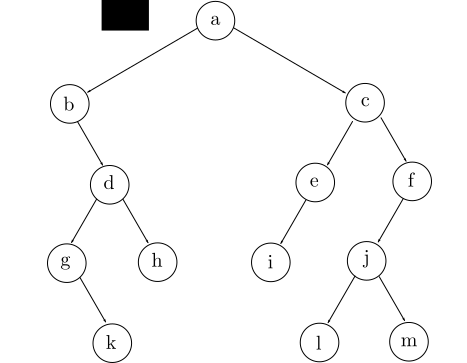
\includegraphics[width=\textwidth]{tree}
\end{figure}

The \emph{root} of the tree is the only node without a parent and so a is the root of this tree. The \emph{leaves} are the nodes without any children, so the leaves of this tree are: k, h, i, l, and m. The \emph{height} of the tree is the longest path from the root to a leaf, and so the height of this tree is 4.

We will now list the nodes of the tree by traversing it in different ways.
\paragraph{Preorder:} We list the node first, then the left and right subtrees recursively.
\begin{center}
\verb+Result:  a, b, d, g, k, h, c, e, i, f, j, l, m+ 
\end{center}
\paragraph{Postorder:} We list the left and right subtrees recursively first, then the node.
\begin{center}
\verb+Result:  k, g, h, d, b, i, e, l, m, j, f, c, a+ 
\end{center}
\paragraph{Inorder:} We list the left subtree, then the node, then the right subtree.
\begin{center}
\verb+Result:  g, k, d, h, b, a, i, e, c, l, j, m, f+ 
\end{center}
\paragraph{Level-order:} We list the nodes from left to right, top to bottom.
\begin{center}
\verb+Result:  a, b, c, d, e, f, g, h, i, j, k, l, m+ 
\end{center}

\section*{Exercise 6 (BST - Insertion and Deletion)}


\end{document}

